% Created 2026-04-23 Thu 12:09
% Intended LaTeX compiler: lualatex
\DocumentMetadata{lang = en-US,pdfversion = 2.0,pdfstandard = ua-2,tagging = on,tagging-setup = {math/setup=mathml-SE},}
\documentclass[11pt]{article}
\usepackage{amsmath}
\usepackage{fontspec}
\usepackage{graphicx}
\usepackage{longtable}
\usepackage{wrapfig}
\usepackage{rotating}
\usepackage[normalem]{ulem}
\usepackage{capt-of}
\usepackage{hyperref}
\usepackage[margin=1in]{geometry}
\usepackage{fontspec}
\usepackage{verbatim, multicol, tabularx,}
\usepackage{amsmath, amsthm, amssymb, stmaryrd, latexsym, bm, listings, qtree}
\usepackage{framed}
\usepackage{xcolor,colortbl}
\usepackage{media9}
\usepackage[export]{adjustbox}
\usepackage{algorithm}
\usepackage[noend]{algpseudocode}
\usepackage{tikz,pgfplots}
\usetikzlibrary{shapes.geometric}
\let\oldquote=\quote
\let\endoldquote=\endquote
\colorlet{shadecolor}{cyan!15}
\renewenvironment{quote}{\begin{shaded*}\begin{oldquote}}{\end{oldquote}\end{shaded*}}
% From https://tex.stackexchange.com/questions/7032/good-way-to-make-textcircled-numbers
\newcommand*\circled[1]{\tikz[baseline=(char.base)]{\node[shape=circle,draw,inner sep=2pt] (char) {#1};}}
\DeclareMathOperator*{\argmin}{arg\!min}
\DeclareMathOperator*{\argmax}{arg\!max}
\lstset{frame=tb, aboveskip=1mm, belowskip=0mm, showstringspaces=false, columns=flexible, basicstyle={\scriptsize\ttfamily}, numbers=left, frame=single, breaklines=true, breakatwhitespace=true}
\hypersetup{colorlinks=true,urlcolor=blue}
\usepackage{tagpdf}
\tagpdfsetup{activate-all}
\tagpdfsetup{math/alt/use}
\usepackage{polyglossia}
\setdefaultlanguage[variant=en-US]{english}
\author{Christopher Simpkins}
\date{Kennesaw State University}
\title{Artificial Intelligence\\\medskip
\large Probabilistic Temporal Reasoning (AIMA 14.1-14.2)}
\hypersetup{
 pdfauthor={Christopher Simpkins},
 pdftitle={Artificial Intelligence},
 pdfkeywords={},
 pdfsubject={Artificial Intelligence Probabilistic Temporal Reasoning (AIMA 14.1-14.2)},
 pdfcreator={Emacs 30.2 (Org mode 9.7.11)}, 
 pdflang={English}}
\begin{document}

\maketitle
\section{Probabilistic Temporal Reasoning}
\label{sec:orgf5dae79}

Recall belief state maintenance from the Kindergarten vacuum world (square not being actively cleaned can become dirty):


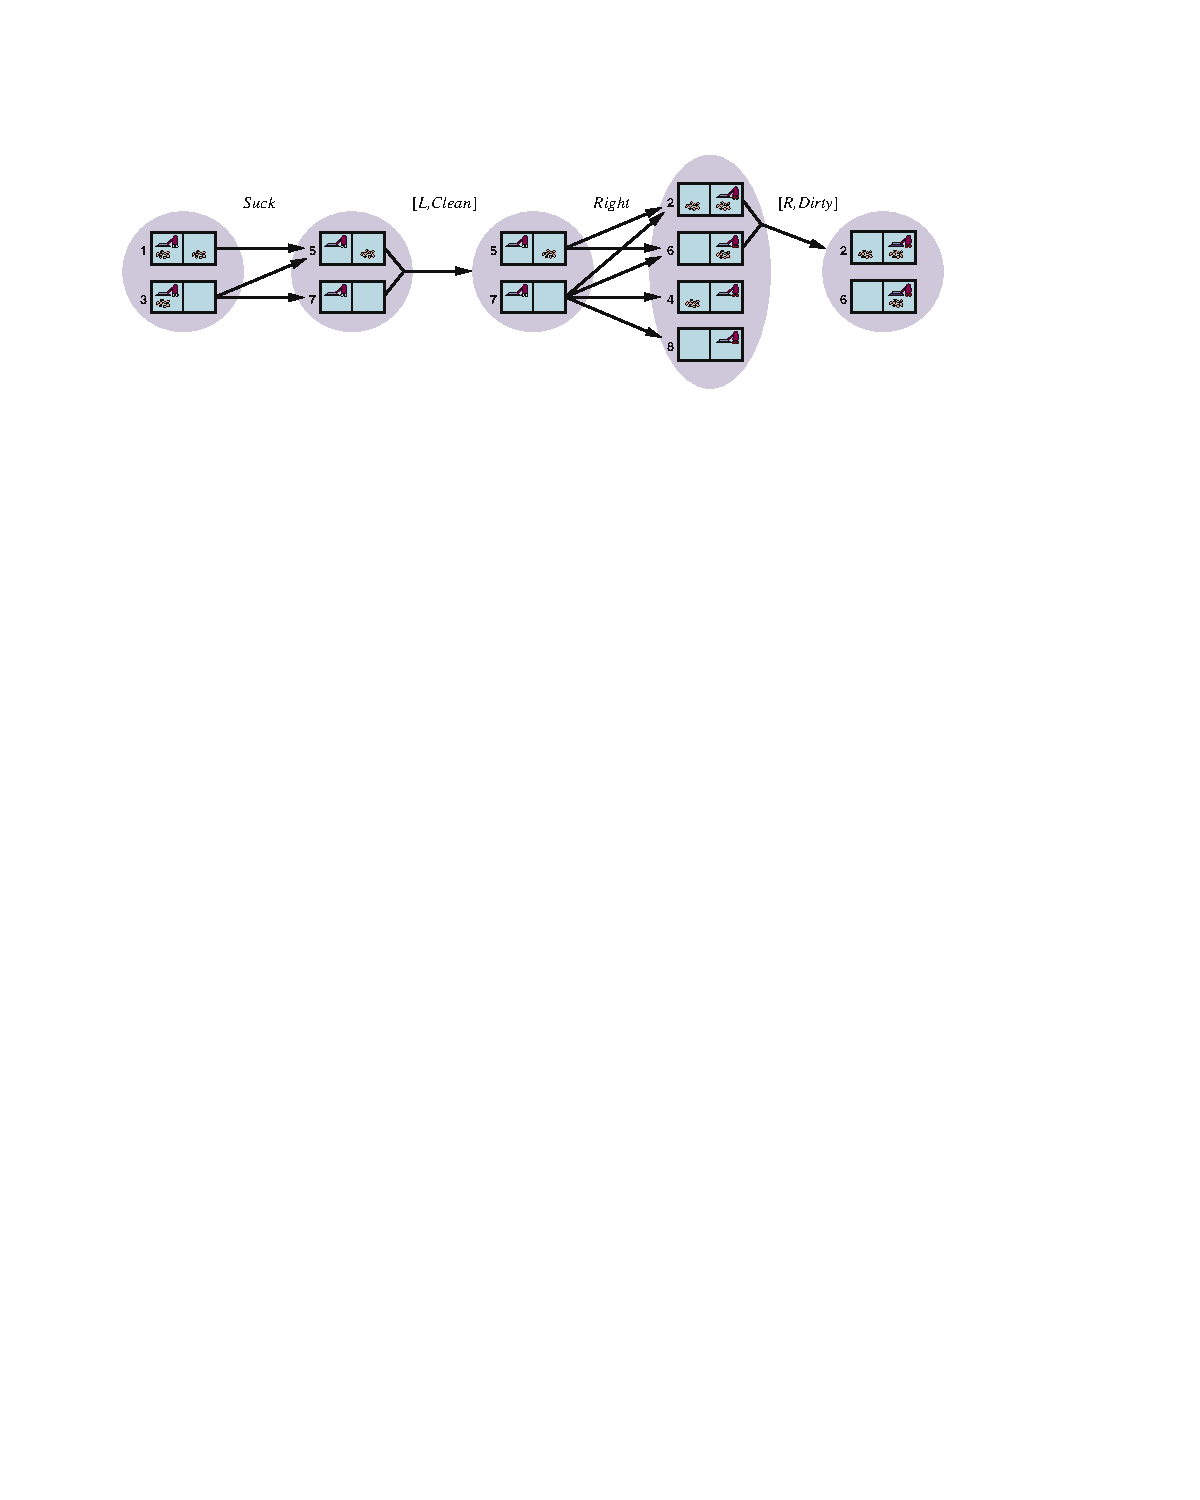
\includegraphics[alt={aima fig 04_17 vacuum prediction update cycles},height=1.2in]{aima-fig-04_17-vacuum-prediction-update-cycles.pdf}


\begin{itemize}
\item Most real-world environments partially observable.  Belief state maintenance is core task.
\item Also known as \textbf{monitoring}, \textbf{filtering}, and \textbf{state estimation}.
\end{itemize}

\begin{equation*}
b' = Update(Predict(b,a),o).
\end{equation*}

\begin{itemize}
\item Equation above is called a recursive state estimator because it computes the new belief state from the previous one rather than by examining the entire percept sequence.
\end{itemize}

Previous methods allowed us to represent belief states as sets of possible worlds, but could not compute or represent how likely these states were.  In this lesson we use the tools of probability theory to quantify our degree of belief in elements of the belief state.
\section{Elements of Stochastic Temporal Models}
\label{sec:org3ef288b}

A changing world is modeled using

\begin{itemize}
\item a variable for each aspect of the world state at each point in time,

\item a transition model describing the probability distribution of the variables at time \(t\), given the state of the world at past times, and

\item a sensor model (a.k.a. observation model) describing the probability of each percept at time \(t\), given the current state of the world.
\end{itemize}
\section{Time and Uncertainty}
\label{sec:org9fb30bf}

Static worlds: each random variable has a single fixed value.

Example: car repair.  Car stays broken during diagnosis.

Dynamic worlds: each random variable has a value for each time step which depends on the values of other random variables in previous time steps.

Example: Diabetes.

\begin{itemize}
\item Task is to assess current state of the patient -- blood sugar and insulin levels -- in order to choose patient's food intake and insulin dose.

\item Blood sugar levels and their measurements can change rapidly over time, depending on recent food intake, insulin doses, metabolic activity, the time of day, and so on.

\item To assess the current state from the history of evidence and predict the outcomes of treatment actions, we must model these changes.
\end{itemize}


Other examples:

\begin{itemize}
\item Robot location tracking
\item Tracking national economic activity
\item Interpreting written or spoken sequences of words
\end{itemize}
\section{Discrete-Time Models}
\label{sec:org9e295f2}

In \textbf{Discrete-time} models:

\begin{itemize}
\item World is a series of snapshots or \textbf{time slices}.
\item Time slices numbered \(0, 1, 2, \dots\)
\item Time interval \(\Delta\) between slides assumed to be the saem for every interval.
\item Particular applications use particular choices of \(\Delta\), e.g., \(\frac{1}{30}\) of a second.
\item Choice of \(\Delta\) should reflect rates of change.

\begin{itemize}
\item E.g., blood glucose can change siginificantly in 10 minutes, so \(\Delta = 1\) minute might be appropriate.
\end{itemize}
\end{itemize}

Discrete vs continuous time:

\begin{itemize}
\item Continuous time systems can be modeled by stochastic differential equations (SDEs).
\item Descrete-time models presented here are approximations to SDEs.
\end{itemize}
\section{States and Observations}
\label{sec:org80b404e}

Each time slice contains a set of random variables:

\begin{itemize}
\item \(\bm{X}_t\) is a set of unobservable state variables at time \(t\).
\item \(\bm{E}_t\) is a set of observable evidence variables at time \(t\).
\end{itemize}

Observation at time \(t\) is \(\bm{E}_t = \bm{e}_t\) for some set of values \(\bm{e}_t\).

\textbf{Example: Security guard in underground facility.}  You are stuck inside with no access to outside world.  Each morning you observe a person walking in with or without an umbrella.

\begin{itemize}
\item \(\Delta\) is one day, each \(t\) is a day.
\item \(\bm{E}_t\) contains a single evidence variable, \(Umbrella_t\) or \(U_t\) for short.
\item \(\bm{X}_t\) contains a single state variable, \(Rain_t\) or \(R_t\) for short.
\end{itemize}

\textbf{Example: diabetes}.

\begin{itemize}
\item \(\bm{E}_t = \{ MeasuredBloodSugar_t, PulseRate_t \}\)
\item \(\bm{X}_t = \{ BloodSugar_t, StomacheContents_t \}\)
\end{itemize}

A few assumptions about \(t\):

\begin{itemize}
\item State sequence starts at time \(t = 0\). (In umbrella world, \(\bm{X} = \{R_0, R_1, R_2, \dots \}\).)
\item Evidence starts arriving at time \(t = 1\). (In umbrella world, \(\bm{E} = \{U_1, U_2, \dots \}\).)
\item \(\bm{X}_{a:b}\) denotes set of variables from \(\bm{X}_a\) to \(\bm{X}_b\), inclusive.

\begin{itemize}
\item Note: inclusive, unlike Python where `U[1:3]` includes only `U[1]` and `U[2]`
\end{itemize}
\end{itemize}
\section{Transition Models}
\label{sec:orgc1e92d0}

The transition model specifies the probability distribution over the latest state variables, given previous values: \(P(\bm{X}_t \mid \bm{X}_{0:t-1})\)

\begin{itemize}
\item Problem: \(\bm{X}_{0:t-1}\) is unbounded -- size increases as \(t\) increases.
\item Solution: \textbf{Markov assumption} -- current state depends on a finite fixed number of previous states.

\begin{itemize}
\item First studied by Andrei Markov (1856-1922), now called \textbf{Markov processes} or \textbf{Markov chains}.
\end{itemize}
\end{itemize}

In these Bayes nets:


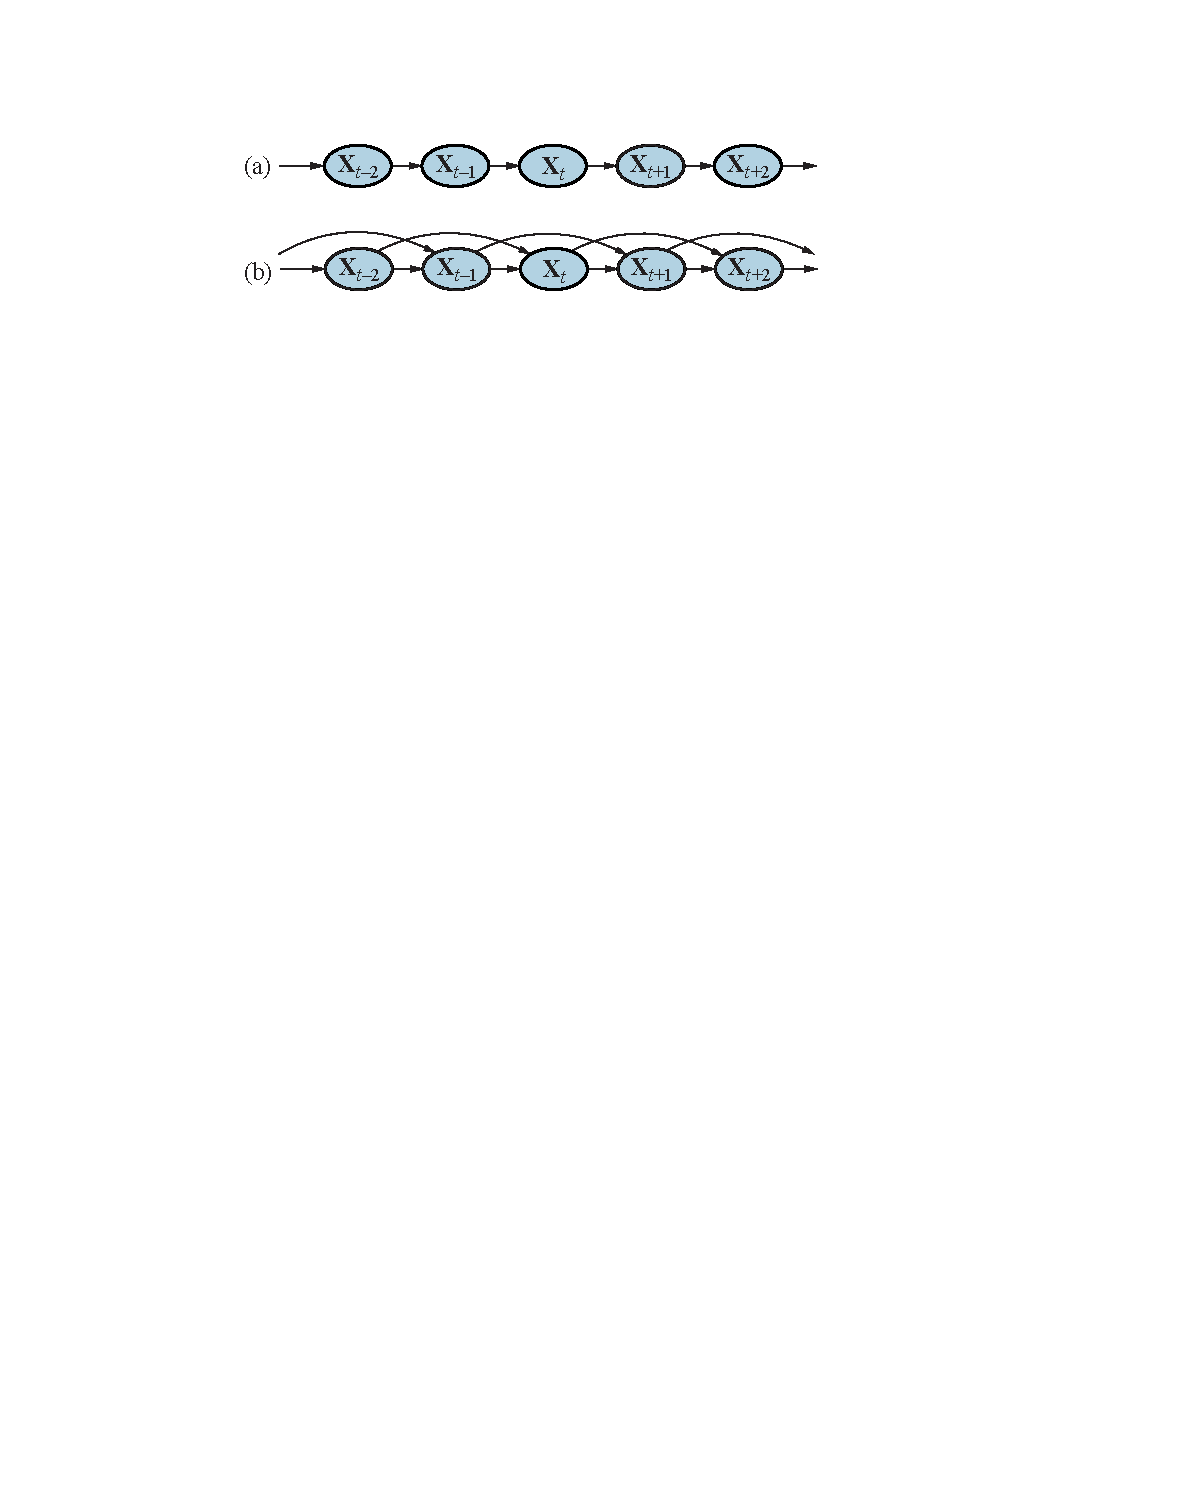
\includegraphics[alt={aima fig 14_01 bayes net markov processes},width=0.75\linewidth]{aima-fig-14_01-bayes-net-markov-processes.pdf}


\begin{itemize}
\item (a) First-order Markov process: \(P(\bm{X}_t \mid \bm{X}_{0:t-1}) = P(\bm{X}_t \mid \bm{X}_{t-1})\)
\item (b) Second-order Markov process: \(P(\bm{X}_t \mid \bm{X}_{0:t-1}) = P(\bm{X}_t \mid \bm{X}_{t-2}, \bm{X}_{t-1})\)
\end{itemize}
\section{Time-Homogeneous Processes}
\label{sec:org18450ca}

Problem:

\begin{itemize}
\item Inifintely many values of \(t\).
\item Could be different distributions for each variable at each time step.
\end{itemize}

Solution: assume \textbf{time homogeneity}, i.e., state changes caused by laws that don't change over time.

Example: Umbrella world

\begin{itemize}
\item \(P(R_t \mid R_{t-1})\) is the same for all \(t\)
\item Only need one conditional probability table.
\end{itemize}
\section{Sensor Models}
\label{sec:org48f6453}

\textbf{Sensor Markov assumption}: state alone is sufficient to generate current sensor values.

\begin{equation*}
P(\bm{E}_t \mid \bm{X}_{0:t}, \bm{E}_{1:t-1}) = P(\bm{E}_t \mid \bm{X}_t) \tag{14.2}
\end{equation*}


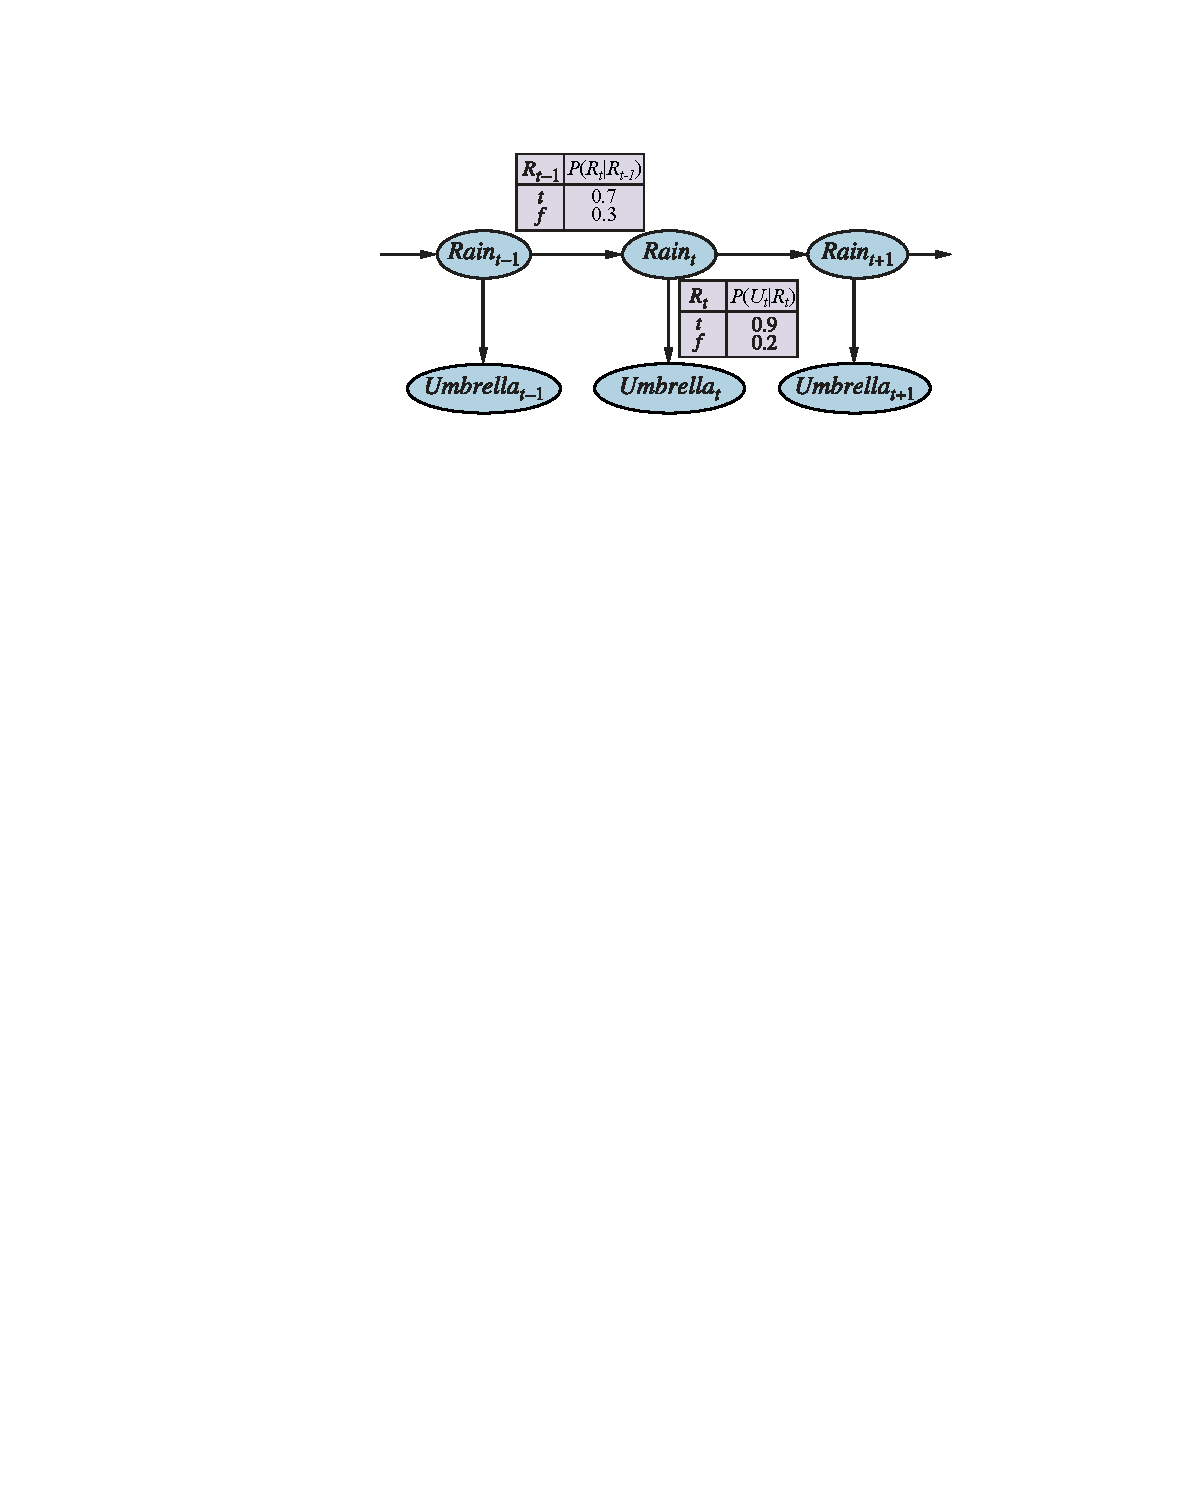
\includegraphics[alt={aima fig 14_02 bayes net umbrella world},height=1.6in]{aima-fig-14_02-bayes-net-umbrella-world.pdf}


\begin{itemize}
\item Transition model is \(P(Rain_t \mid Rain_{t-1})\).
\item Sensor model is \(P(Umbrella_t \mid Rain_t)\).
\item Arrows go from actual state to sensor values: states \textbf{cause} sensor values.

\begin{itemize}
\item Inference goes in other direction: given sensor values, what are the state values.
\end{itemize}
\end{itemize}
\section{Full Joint Distribution Over All Variables in a Temporal Model}
\label{sec:orgf4a7fe9}

For the initial state of the system at time \(0\) we specify a prior \(P(\bm{x}_0)\).  Now we can use Equation 13.2

\begin{equation*}
P(x_1, \dots, x_n) = \prod_{i=1}^n P( x_i | parents(X_i)) \tag{13.2}
\end{equation*}

applied to the temporal variables in the dynamic version:

\begin{equation*}
P(\bm{X}_{0:t}, \bm{E}_{1:t}) = \underbrace{P(\bm{X}_0)}_{\text{Initial state model}} \prod_{i=1}^t \underbrace{P(\bm{X}_i \mid \bm{X}_{i-1})}_{\text{Transition model}} \underbrace{P(\bm{E}_i \mid \bm{X}_i)}_{\text{Sensor model}} \tag{14.3}
\end{equation*}

Standard Bayes nets can only represent a finite set of variables.  Dynamic Bayes nets overcome this limitation by:

\begin{itemize}
\item defining infinite sets by integer indices, and
\item using implicit universal quantification to define sensor and transition models for every time step.
\end{itemize}
\section{Markov Model Considerations}
\label{sec:org0a78957}

Sometimes Markov assumption is valid, sometimes it's only an approximation.  Two ways to improve the approximation:

\begin{enumerate}
\item Increase the order of the Markov process model.  E.g., In Palo Alto, CA, rarely rains more than two days in a row.  A 2nd-order Markov model could express this fact:

\item \(P(r_t \mid r_{t-1}, r_{t-2}) \ll P(r_t \mid r_{t-1}, \neg r_{t-2})\).

\item Add additional state variables.  E.g., add \(Season_t\) for hisotircal records, or \(Temperature_t\), \(Humidity_t\), and \(Pressure_t\) to use a physical model of rainy conditions.
\end{enumerate}
\section{Example: Battery Drainage in a Mobile Robot}
\label{sec:orgbd61434}

Two state variables: velocity and position.  Use Newton's laws of motion to calculate new positions.  Add probabilistic error (e.g., Gaussian noise) to account for uncertainty in velocity due to terrain, wind, etc.

Problems:

\begin{itemize}
\item Battery level affects velocity as it drains.
\item Battery level depends on power used in all previous movements, violating the Markov assumption.
\end{itemize}

Solution: Add a state variable for battery level.  Track level in one of two ways:

\begin{enumerate}
\item Decrease level at each time step in response to movement executed in previous step.
\item Better: add a new sensor for battery level.
\end{enumerate}
\section{Inference in Temporal Models}
\label{sec:org50777b6}

Given the general structure of a probabilistic temporal model, we can perform basic inference tasks:

\begin{itemize}
\item \textbf{Filtering}, a.k.a., \textbf{state estimation} is the task of computing the \textbf{belief state} \(P(\bm{X}_t \mid \bm{e}_{1:t})\) -- the posterior distribution over the most recent state given all the evidence to date.

\item \textbf{Prediction} is the task of computing the posterior distribution over the future state, given all evidence to date: \(P(\bm{X}_{t+k} \mid \bm{e}_{1:t})\) for some \(k > 0\).

\item \textbf{Smoothing} is the task of computing the posterior distribution over a past state, given all evidence up to the present: \(P(\bm{X}_k \mid \bm{e}_{1:t})\) for some \(k\) such that \(0 \le k < t\).

\item \textbf{Most likely explanation}: Given a sequence of observations, we might wish to find the sequence of states that is most likely to have generated those observations: \(\argmax_{x_{1:t}} P(\bm{x}_{1:t} \mid \bm{e}_{1:t})\).
\end{itemize}
\section{Learning Temporal Models}
\label{sec:orgfcec186}

Unknown transition and sensor models can be learned from observations.

\begin{itemize}
\item As with static Bayesian networks, dynamic Bayes net learning can be done as a by-product of inference.

\item Inference provides an estimate of transitions that actually occurred and the states that generated the sensor readings, and these estimates can be used to learn the models.

\item Learning via iterative update algorithm, expectation–maximization or EM, or Bayesian updating of the model parameters given the evidence.
\end{itemize}

We'll return to these ideas in our lesson on statistical learning.
\section{Filtering}
\label{sec:org89665b7}

\textbf{Filtering}, a.k.a., \textbf{state estimation} is the task of computing the \textbf{belief state} \(P(\bm{X}_t \mid \bm{e}_{1:t})\) -- the posterior distribution over the most recent state given all the evidence to date.

\begin{itemize}
\item Umbrella example: compute probability of rain today given all umbrella observations so far.
\item Rational agent estimates its current state to enable rational decisions.
\item Nearly identical calculation provides likelihood of evidence sequence \(P(\bm{e}_{1:t})\)
\item The term "filtering" comes from signal processing, which sees the problem of state estimation as "filtering out the noise" in a signal to estimate its underlying properties.
\end{itemize}

\textbf{Need for efficiency.} A useful filtering algorithm needs to maintain a current state estimate and update it, rather than going back over the entire history of percepts for each update.

\begin{itemize}
\item Otherwise, the cost of each update increases as time goes by.
\end{itemize}

In other words, given the result of filtering up to time \(t\), the agent needs to compute the result for \(t + 1\) from the new evidence \(\bm{e}_{t+1}\).  For some function \(f\):

\begin{equation*}
P(\bm{X}_{t+1} \mid f \left( \bm{e}_{t+1}, P(\bm{X}_t \mid \bm{e}_{1:t}) \right)
\end{equation*}
\section{Recursive State Estimation}
\label{sec:orgb7aa51e}

We can view the calculation as being composed of two parts: first, the current state distribution is projected forward from \(t\) to \(t + 1\); then it is updated using the new evidence \(\bm{e}_{t+1}\). This two-part process emerges quite simply when the formula is rearranged:

\vspace{-.25in}
\begin{align*}
P(\bm{X}_{t+1} \mid \bm{e}_{1:t+1}) &= P(\bm{X}_{t+1} \mid \bm{e}_{1:t}, \bm{e}_{t+1}) \tag{Divide the evidence}\\
                                     &= \alpha P(\bm{e}_{t+1} \mid \bm{X}_{t+1}, e_{1:t}) P(\bm{X}_{t+1} \mid \bm{e}_{1:t}) \tag{Bayes rule, given $\bm{e}_{1:t}$}\\
                                     &= \alpha \underbrace{P(\bm{e}_{t+1} \mid \bm{X}_{t+1})}_{\text{update}} \underbrace{P(\bm{X}_{t+1} \mid \bm{e}_{1:t})}_{\text{prediction}} \tag{Sensor Markov assumption}
\end{align*}

Now plug in an expression for one-step prediction \(P(\bm{X}_{t+1} \mid \bm{e}_{1:t})\) conditioned on the current state \(\bm{X}_t\) to obtain the central result in probabilistic temoral reasoning:

\vspace{-.25in}
\begin{align*}
P(\bm{X}_{t+1} \mid \bm{e}_{1:t+1}) &= \alpha P(\bm{e}_{t+1} \mid \bm{X}_{t+1}) \sum_{\bm{X}_t} P(\bm{X}_{t+1} \mid \bm{x}_t, \bm{e}_{1:t}) P(\bm{x}_t \mid \bm{e}_{1:t}) \\
                                     &= \alpha \underbrace{P(\bm{e}_{t+1} \mid \bm{X}_{t+1})}_{\text{sensor model}} \sum_{\bm{X}_t} \underbrace{P(\bm{X}_{t+1} \mid \bm{x}_t)}_{\text{transition model}} \underbrace{P(\bm{x}_t \mid \bm{e}_{1:t})}_{\text{recursion}} \tag{14.5}
\end{align*}

The last step applies the Markov assumption in the transition model.  All the terms come either from the model or from the previous state estimate.
Hence, we have the desired recursive formulation.
\section{Forward Message Propagation}
\label{sec:org124e659}

\vspace{-.2in}
\[
P(\bm{X}_{t+1} \mid \bm{e}_{1:t+1}) = \alpha \underbrace{P(\bm{e}_{t+1} \mid \bm{X}_{t+1})}_{\text{sensor model}} \sum_{\bm{X}_t} \underbrace{P(\bm{X}_{t+1} \mid \bm{x}_t)}_{\text{transition model}} \underbrace{P(\bm{x}_t \mid \bm{e}_{1:t})}_{\text{recursion}} \tag{14.5}
\]

We can think of the filtered estimate \(P(\bm{X}_t \mid \bm{e}_{1:t})\) as a "message" \(\bm{f}_{1:t}\) that is propagated forward along the sequence, modified by each transition and updated by each new observation. The process is given by

\begin{equation*}
\bm{f}_{1:t+1} = \text{FORWARD}(\bm{f}_{1:t}, \bm{e}_{t+1})
\end{equation*}

where

\begin{itemize}
\item FORWARD implements the update in Equation 14.5 and
\item the process begins with \(\bm{f}_{1:0} = P(\bm{X}_0)\).
\end{itemize}

When all the state variables are discrete, the time for each update is constant (i.e., independent of \(t\)), and the space required is also constant. (The constants depend, of course, on the size of the state space and the specific type of the temporal model in question.)

\begin{itemize}
\item \textbf{The time and space requirements for updating must be constant if a finite agent is to keep track of the current state distribution indefinitely}.
\end{itemize}
\section{Example: Filtering in the Umbrella World}
\label{sec:orgf9e840f}





Compute \(P(R_2 \mid u_{1:2})\):

\begin{itemize}
\item Day 0: no observations, only prior beliefs: \(P(R_0) = \langle 0.5, 0.5 \rangle\)
\item Day 1: umbrealla appears, \(U_1 = true\).  Prediction from \(t=0:1\):

```\{=latex\}
\vspace{-.2in}
\begin{align*}
P(R_1) &= \sum_{r_0} P(R_1 \mid r_0) P(r_0) \\
        &= \langle 0.7, 0.3 \rangle \cdot 0.5 + \langle 0.3, 0.7 \rangle \cdot 0.5 \\
        &= \langle 0.5, 0.5 \rangle
\end{align*}
```

Then update step incorporates evidence for \(t=1\) and normalizes:

```\{=latex\}
\vspace{-.2in}
\begin{align*}
P(R_1 \mid u_1) &= \alpha P(u_1 \mid R_1) P(R_1) \\
                 &= \alpha \langle 0.9, 0.2 \rangle \langle 0.5, 0.5 \rangle \\
                 &= \alpha \langle 0.45, 0.1 \rangle \\
                 &\approx \langle 0.818, 0.182 \rangle
\end{align*}
```
\end{itemize}




\vspace{-.2in}

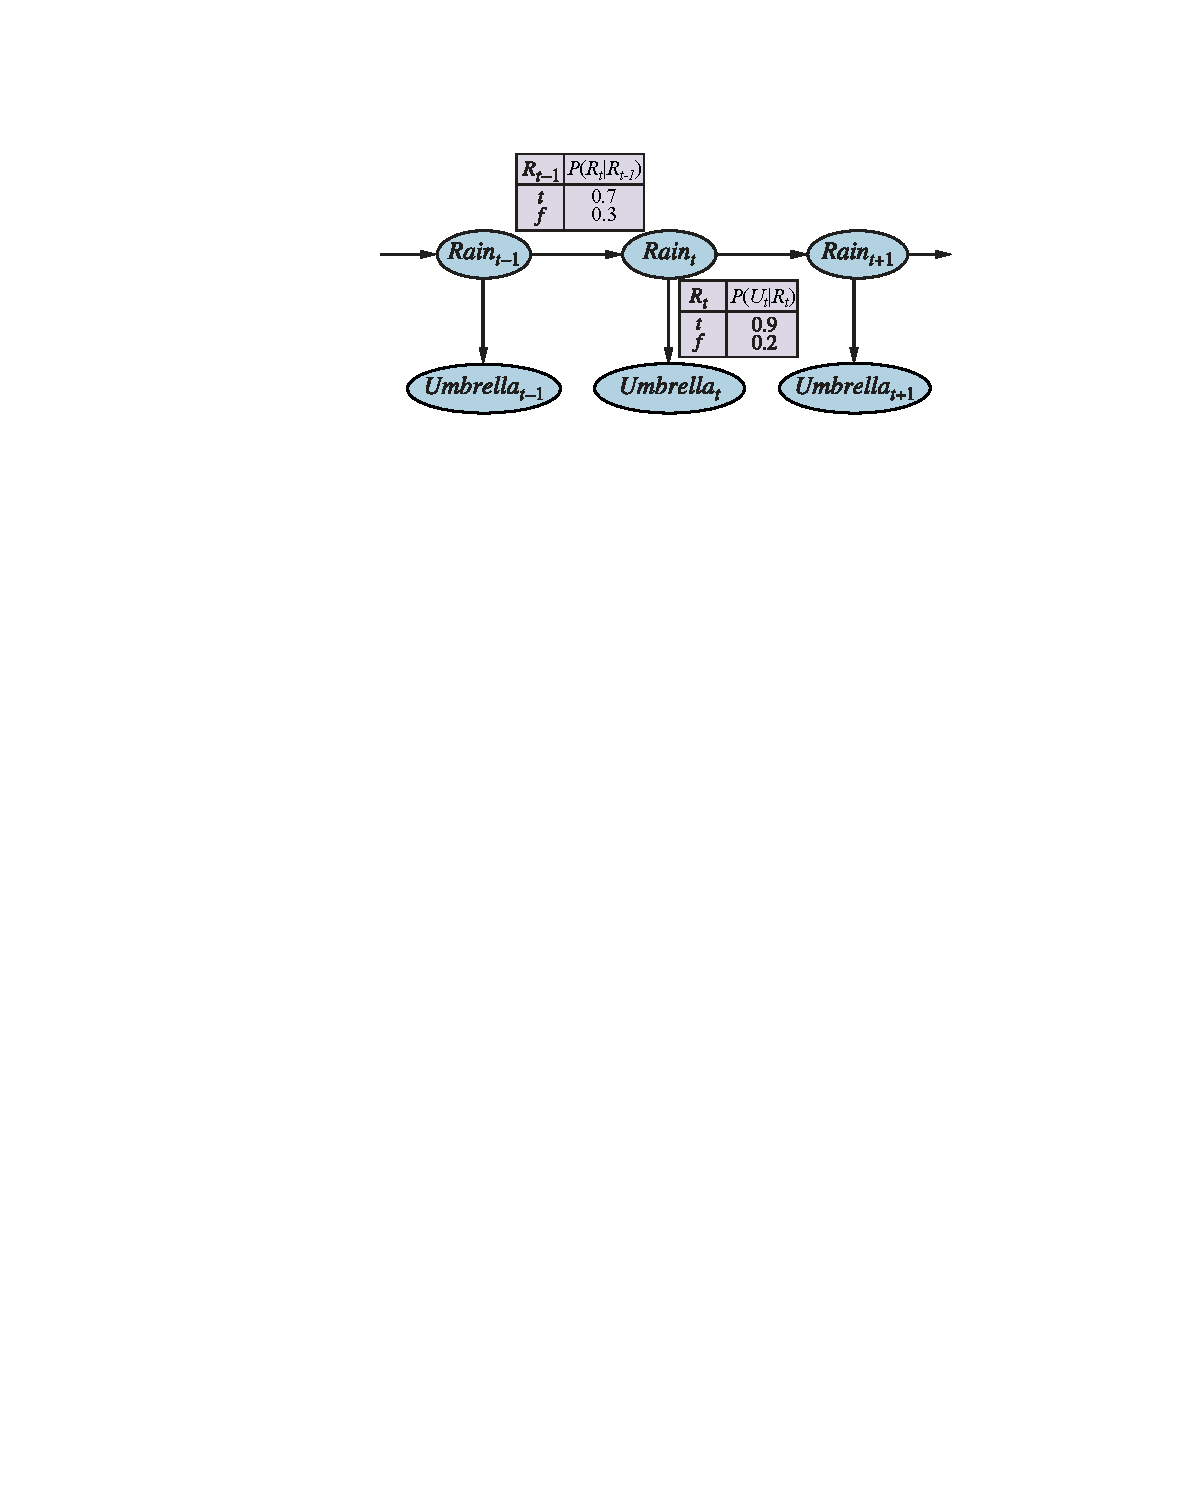
\includegraphics[alt={aima fig 14_02 bayes net umbrella world},height=1.0in]{aima-fig-14_02-bayes-net-umbrella-world.pdf}


\begin{itemize}
\item Day 2: umbrella appears, \(U_2 = true\).  Prediction from \(t=1:2\):

```\{=latex\}
\vspace{-.2in}
\begin{align*}
P(R_2 \mid u_1) &= \sum_{r_1} P(R_2 \mid r_1) P(r_1 \mid u_1) \\
                 &= \langle 0.7, 0.3 \rangle \cdot 0.818 + \langle 0.3, 0.7 \rangle \cdot 0.182 \\
                 &\approx \langle 0.627, 0.373 \rangle
\end{align*}
```

Then update step incorporates evidence for \(t=2\):

```\{=latex\}
\vspace{-.2in}
\begin{align*}
P(R_2 \mid u_1, u_2) &= \alpha P(u_2 \mid R_2) P(R_2 \mid u_1) \\
                      &= \alpha \langle 0.9, 0.2 \rangle \langle 0.627, 0.373 \rangle \\
                      &= \alpha \langle 0.565, 0.075 \rangle \\
                      &\approx \langle 0.883, 0.117 \rangle
\end{align*}
```
\end{itemize}
\section{Inference in Temporal Models}
\label{sec:org364c54c}

Given the general structure of a probabilistic temporal model, we can perform basic inference tasks:

\begin{itemize}
\item \textbf{Filtering}, a.k.a., \textbf{state estimation} is the task of computing the \textbf{belief state} \(P(\bm{X}_t \mid \bm{e}_{1:t})\) -- the posterior distribution over the most recent state given all the evidence to date.
\end{itemize}

\fbox\{
\begin{minipage}{\textwidth}
\begin{itemize}
\item {\bf Prediction} is the task of computing the posterior distribution over the future state, given all evidence to date: $P(\bm{X}_{t+k} \mid \bm{e}_{1:t})$ for some $k > 0$.
\end{itemize}
\end{minipage}
\}
\begin{itemize}
\item \textbf{Smoothing} is the task of computing the posterior distribution over a past state, given all evidence up to the present: \(P(\bm{X}_k \mid \bm{e}_{1:t})\) for some \(k\) such that \(0 \le k < t\).

\item \textbf{Most likely explanation}: Given a sequence of observations, we might wish to find the sequence of states that is most likely to have generated those observations: \(\argmax_{x_{1:t}} P(\bm{x}_{1:t} \mid \bm{e}_{1:t})\).
\end{itemize}
\section{Prediction}
\label{sec:org24210d9}

\textbf{Prediction} is the task of computing the posterior distribution over the future state, given all evidence to date: \(P(\bm{X}_{t+k} \mid \bm{e}_{1:t})\) for some \(k > 0\).

\begin{itemize}
\item Umbrella example: compute probability of rain three days from now, given all the observations to date.
\item Prediction is useful for evaluating possible courses of action based on their expected outcomes.
\end{itemize}


Prediction can be seen simply as filtering without the addition of new evidence.  Filtering already includes a one-step prediciton.  So we can take Equation 14.5:

\vspace{-.1in}
\[
P(\bm{X}_{t+1} \mid \bm{e}_{1:t+1}) = \alpha \underbrace{P(\bm{e}_{t+1} \mid \bm{X}_{t+1})}_{\text{sensor model}} \sum_{\bm{X}_t} \underbrace{P(\bm{X}_{t+1} \mid \bm{x}_t)}_{\text{transition model}} \underbrace{P(\bm{x}_t \mid \bm{e}_{1:t})}_{\text{recursion}} \tag{14.5}
\]

remove the sensor model and extend the prediction to \(t + k + 1\):

\vspace{-.1in}
\[
P(\bm{X}_{t+k+1} \mid \bm{e}_{1:t}) =  \sum_{\bm{X}_{t+k}} \underbrace{P(\bm{X}_{t+k+1} \mid \bm{x}_{t+k})}_{\text{transition model}} \underbrace{P(\bm{x}_{t+k} \mid \bm{e}_{1:t})}_{\text{recursion}} \tag{14.6}
\]
\section{Making predictions is hard, especially about the future.}
\label{sec:org8ef2858}

As we try to predict further and further into the future, the predicted distribution for rain converges to a fixed point \(\langle 0.5,0.5 \rangle\), after which it remains constant for all time.

\begin{itemize}
\item This is the \textbf{stationary distribution} of the Markov process defined by the transition model.

\item The \textbf{mixing time} is the time it takes to reach the fixed point.

\item Prediction usually only effective for \(k \ll\) mixing time.
\end{itemize}

The more the uncertainty in the transition model, the shorter will be the mixing time and the more the future is obscured.
\section{Inference in Temporal Models}
\label{sec:org6a1fdfd}

Given the general structure of a probabilistic temporal model, we can perform basic inference tasks:

\begin{itemize}
\item \textbf{Filtering}, a.k.a., \textbf{state estimation} is the task of computing the \textbf{belief state} \(P(\bm{X}_t \mid \bm{e}_{1:t})\) -- the posterior distribution over the most recent state given all the evidence to date.

\item \textbf{Prediction} is the task of computing the posterior distribution over the future state, given all evidence to date: \(P(\bm{X}_{t+k} \mid \bm{e}_{1:t})\) for some \(k > 0\).
\end{itemize}

\framebox\{
\begin{minipage}{\textwidth}
\begin{itemize}
\item {\bf Smoothing} is the task of computing the posterior distribution over a past state, given all evidence up to the present: $P(\bm{X}_k \mid \bm{e}_{1:t})$ for some $k$ such that $0 \le k < t$.
\end{itemize}
\end{minipage}
\}

\begin{itemize}
\item \textbf{Most likely explanation}: Given a sequence of observations, we might wish to find the sequence of states that is most likely to have generated those observations: \(\argmax_{x_{1:t}} P(\bm{x}_{1:t} \mid \bm{e}_{1:t})\).
\end{itemize}
\section{Smoothing}
\label{sec:orgad337d6}

\textbf{Smoothing} is the task of computing the posterior distribution over a past state, given all evidence up to the present: \(P(\bm{X}_k \mid \bm{e}_{1:t})\) for some \(k\) such that \(0 \le k < t\).



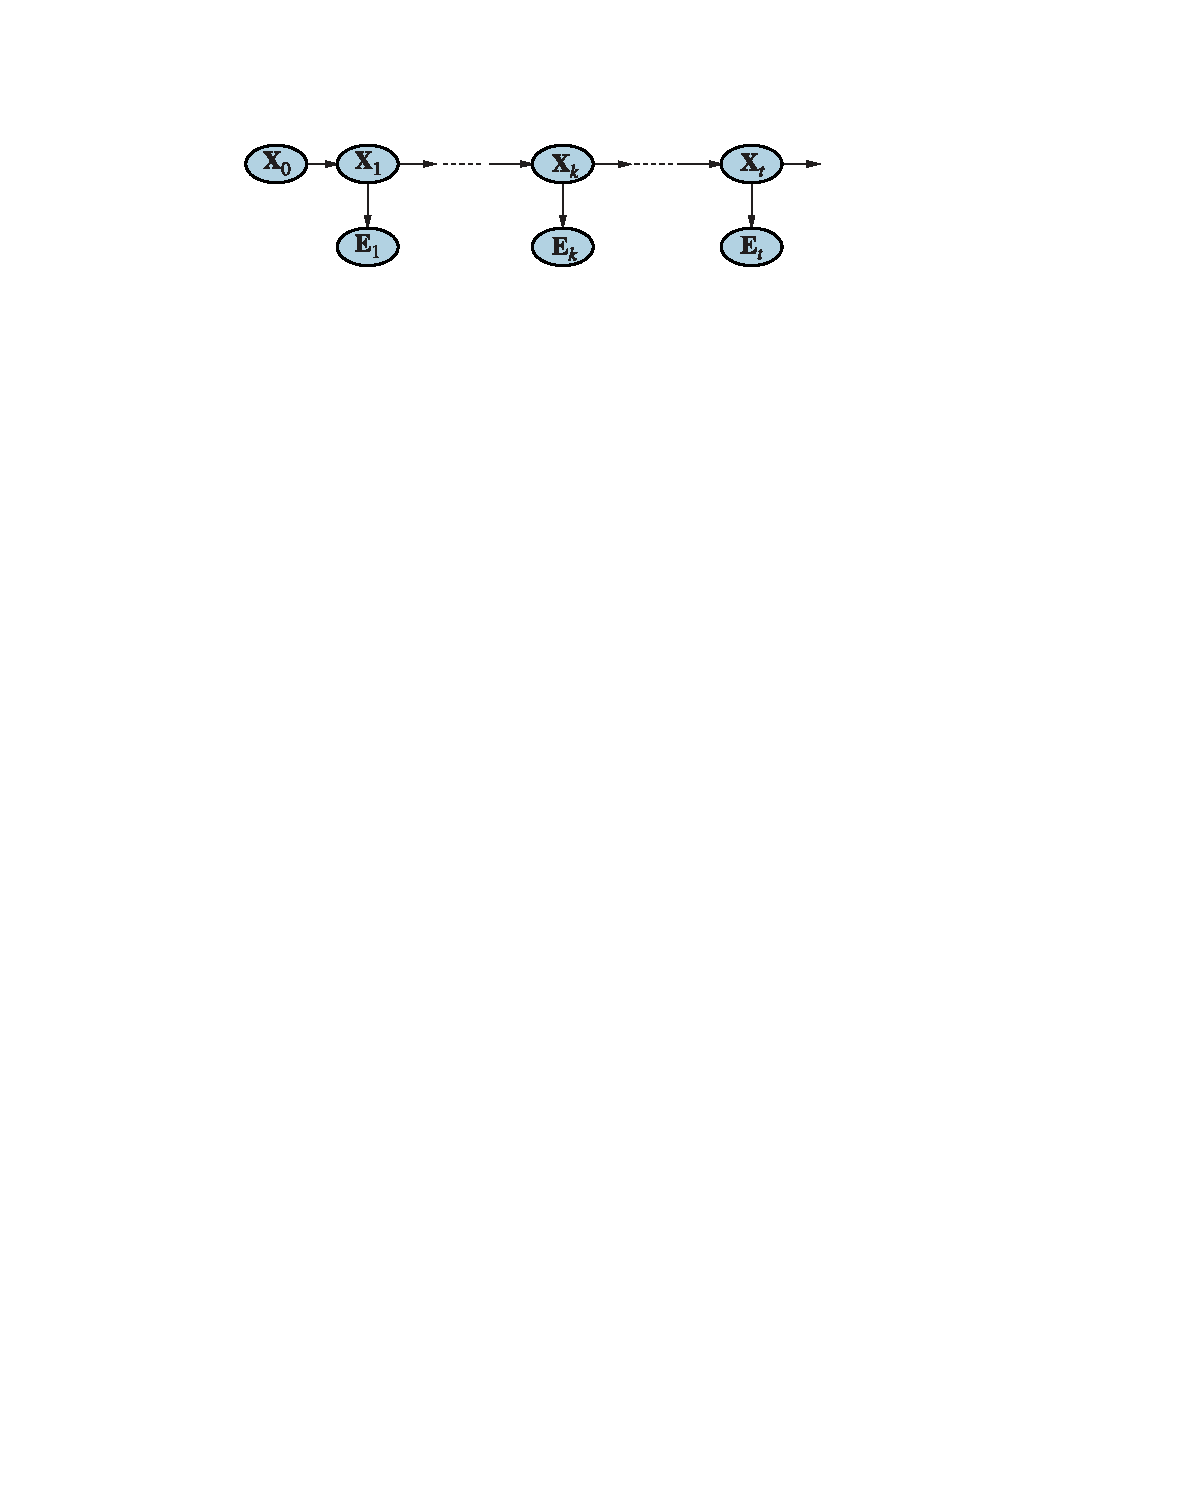
\includegraphics[alt={aima fig 14_03 smoothing},width=0.75\linewidth]{aima-fig-14_03-smoothing.pdf}



\begin{itemize}
\item Umbrella example: compute the probability that it rained last Wednesday, given all the observations of the umbrella carrier made up to today.
\item Smoothing provides a better estimate of the state at time \(k\) than was available at that time, because it incorporates more evidence.

\begin{itemize}
\item When tracking a moving object with inaccurate position observations, smoothing gives a smoother
\end{itemize}
\end{itemize}
estimated trajectory than filtering -- hence the name
\section{Recursive Message Passing for Smoothing}
\label{sec:orgaa5f69a}

Split the computation into two parts -- the evidence up to \(k\) and the evidence from \(k + 1\) to \(t\):

\vspace{-.2in}
\begin{align*}
P(\bm{X}_{k} \mid \bm{e}_{1:t}) &= P(\bm{X}_{k} \mid \bm{e}_{1:k}, \bm{e}_{k+1:t}) \\
                                 &= \alpha P(\bm{X}_k \mid \bm{e}_{1:k}) P(\bm{e}_{k+1:t} \mid \bm{X}_k, \bm{e}_{1:k}) \tag{using Bayes' Rule, given $\bm{e}_{1:k}$} \\
                                 &= \alpha P(\bm{X}_k \mid \bm{e}_{1:k}) P(\bm{e}_{k+1:t} \mid \bm{X}_k) \tag{using conditional indepenence} \\
                                 &= \alpha \bm{f}_{1:k} \odot \bm{b}_{k+1:t} \tag{14.8}
\end{align*}

\(\odot\) is elementwise multiplication, a.k.a. Hadamard product.

The "forward" message, \(\bm{f}_{1:k}\) can be computed by filtering forward using Equation 14.5.

\[
P(\bm{X}_{t+1} \mid \bm{e}_{1:t+1}) = \alpha \underbrace{P(\bm{e}_{t+1} \mid \bm{X}_{t+1})}_{\text{sensor model}} \sum_{\bm{X}_t} \underbrace{P(\bm{X}_{t+1} \mid \bm{x}_t)}_{\text{transition model}} \underbrace{P(\bm{x}_t \mid \bm{e}_{1:t})}_{\text{recursion}} \tag{14.5}
\]
\section{Backward Message for Smoothing}
\label{sec:org989b45b}

The backward message, \(\bm{b}_{k+1:t}\) can be computed by a recursive process running backward from \(t\):

\vspace{-.2in}
\begin{align*}
P(\bm{e}_{k+1:t} \mid \bm{X}_k) &= \sum_{\bm{x}_{k+1}} P(\bm{e}_{k+1:t} \mid \bm{X}_k, \bm{x}_{k+1}) P(\bm{x}_{k+1} \mid \bm{X}_k) \tag{conditioning on $\bm{X}_{k+1}$} \\
                                 &= \sum_{\bm{x}_{k+1}} P(\bm{e}_{k+1:t} \mid \bm{x}_{k+1}) P(\bm{x}_{k+1} \mid \bm{X}_k) \tag{by conditional independence} \\
                                 &= \sum_{\bm{x}_{k+1}} P(\bm{e}_{k+1}, \bm{e}_{k+2:t} \mid \bm{x}_{k+1}) P(\bm{x}_{k+1} \mid \bm{X}_k) \\
                                 &= \sum_{\bm{x}_{k+1}} \underbrace{P(\bm{e}_{k+1} \mid \bm{x}_{k+1})}_{\text{sensor model}} \underbrace{P(\bm{e}_{k+2:t} \mid \bm{x}_{k+1})}_{\text{recursion}} \underbrace{P(\bm{x}_{k+1} \mid \bm{X}_k)}_{\text{transition model}} \tag{14.9}
\end{align*}

The last step follows by the conditional independence of \(\bm{e}_{k+1}\) and \(\bm{e}_{k+2:t}\), given \(\bm{x}_{k+1}\).

Equation 14.9 in message form is

\begin{equation*}
\bm{b}_{k+1:t} = \text{BACKWARD}(\bm{b}_{k+2:t}, \bm{e}_{k+1}).
\end{equation*}

\(\bm{e}_{t+1:t}\) is an empty sequence, so we initialize the backward phase with \(\bm{b}_{t+1:t} = P(\bm{e}_{t+1:t} \mid \bm{X}_t) = \bm{1}\), where \(\bm{1}\) is a vector of 1s.
\section{Example: Smoothed Umbrella World State Estimate}
\label{sec:orgd7c9485}




Let's compute the smoothed estimate for the probability of rain at time \(k = 1\), given the umbrella observations on days 1 and 2.

\vspace{-.2in}
\begin{align*}
P(\bm{X}_{k} \mid \bm{e}_{1:t}) &= \alpha P(\bm{X}_k \mid \bm{e}_{1:k}) P(\bm{e}_{k+1:t} \mid \bm{X}_k) \tag{14.8}\\
P(R_1 \mid u_1, u_2)            &= \alpha P(R_1 \mid u_1) P(u_2 \mid R_1) \tag{14.10}
\end{align*}




\vspace{-.1in}

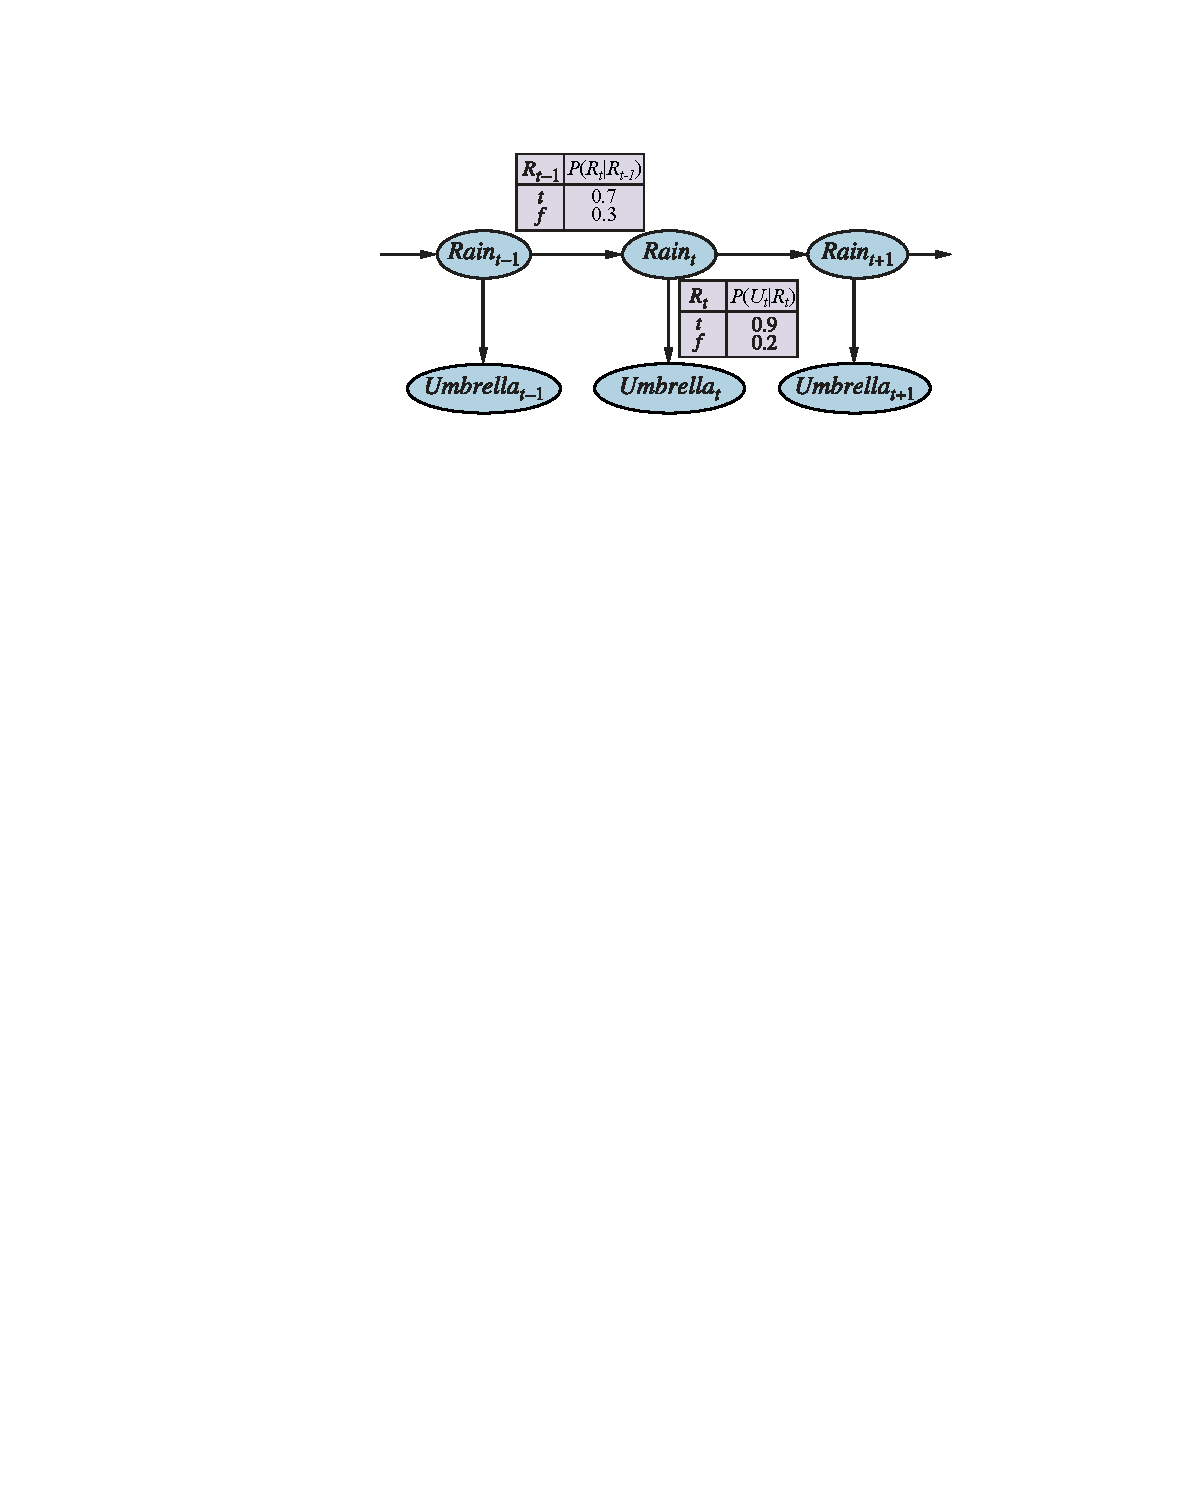
\includegraphics[alt={aima fig 14_02 bayes net umbrella world},height=1.2in]{aima-fig-14_02-bayes-net-umbrella-world.pdf}






From filtering for Day 1 we already know \(P(R_1 \mid u_1) = \alpha P(u_1 \mid R_1) P(R_1) = \langle 0.818, 0.182 \rangle\).

So then we need to compute \(P(u_2 \mid R_1)\) by applying the backward recursion in Equation 14.9:

\vspace{-.2in}
\begin{align*}
P(\bm{e}_{k+1:t} \mid \bm{X}_k) &= \sum_{\bm{x}_{k+1}} P(\bm{e}_{k+1} \mid \bm{x}_{k+1}) P(\bm{e}_{k+2:t} \mid \bm{x}_{k+1}) P(\bm{x}_{k+1} \mid \bm{X}_k) \tag{14.9}\\
P(u_2 \mid R_1)                 &= \sum_{\bm{r}_{2}} P(u_2 \mid r_2) P( \mid r_2) P(r_2 \mid R_1) \\
                                 &= \left( 0.9 \cdot 1 \cdot \langle 0.7, 0.3 \rangle \right) + \left( 0.2 \cdot 1 \cdot \langle 0.3, 0.7 \rangle \right) = \langle 0.69, 0.41 \rangle
\end{align*}

Then plug both terms into Equation 14.10:

\vspace{-.2in}
\begin{align*}
P(R_1 \mid u_1, u_2) &= \alpha P(R_1 \mid u_1) P(u_2 \mid R_1) \tag{14.10} \\
                      &= \alpha \langle 0.818, 0.182 \rangle \odot \langle 0.69, 0.41 \rangle \approx \langle 0.883, 0.117 \rangle
\end{align*}

Knowing it rained on Day 2 makes it more likely that it rained on Day 1.
\section{Complexity of Smoothing}
\label{sec:org8d62cc5}

The forward and backward recursions each take constant time per step.  So:

\begin{itemize}
\item The time complexity of smoothing with respect to evidence \(\bm{e}_{1:t}\) is \(O(t)\) -- the complexity for smoothing at a particular time step \(k\).

\item If we want to smooth the whole sequence, we could run the whole smoothing process once for each time step -- a time complexity of \(O(t^2)\).
\end{itemize}

However, we can apply dynamic programming to reduce the complexity to \(O(t)\).

\begin{itemize}
\item Recall that we reused the results of the forward-filtering phase in our smoothing calculations.

\item The key to the linear-time algorithm is to record the results of forward filtering over the whole sequence.

\item Then we run the backward recursion from \(t\) down to 1, computing the smoothed estimate at each step \(k\) from the computed backward message \(\bm{b}_{k+1:t}\) and the stored forward message \(\bm{f}_{1:k}\).
\end{itemize}

This is the essence of the forward–backward smoothing algorithm \ldots{}

\begin{itemize}
\item BTW, you'll see this algorithmic structure again when you learn about deep neural networks.
\end{itemize}
\section{Forward-Backward Smoothing Algorithm}
\label{sec:org35c42dd}


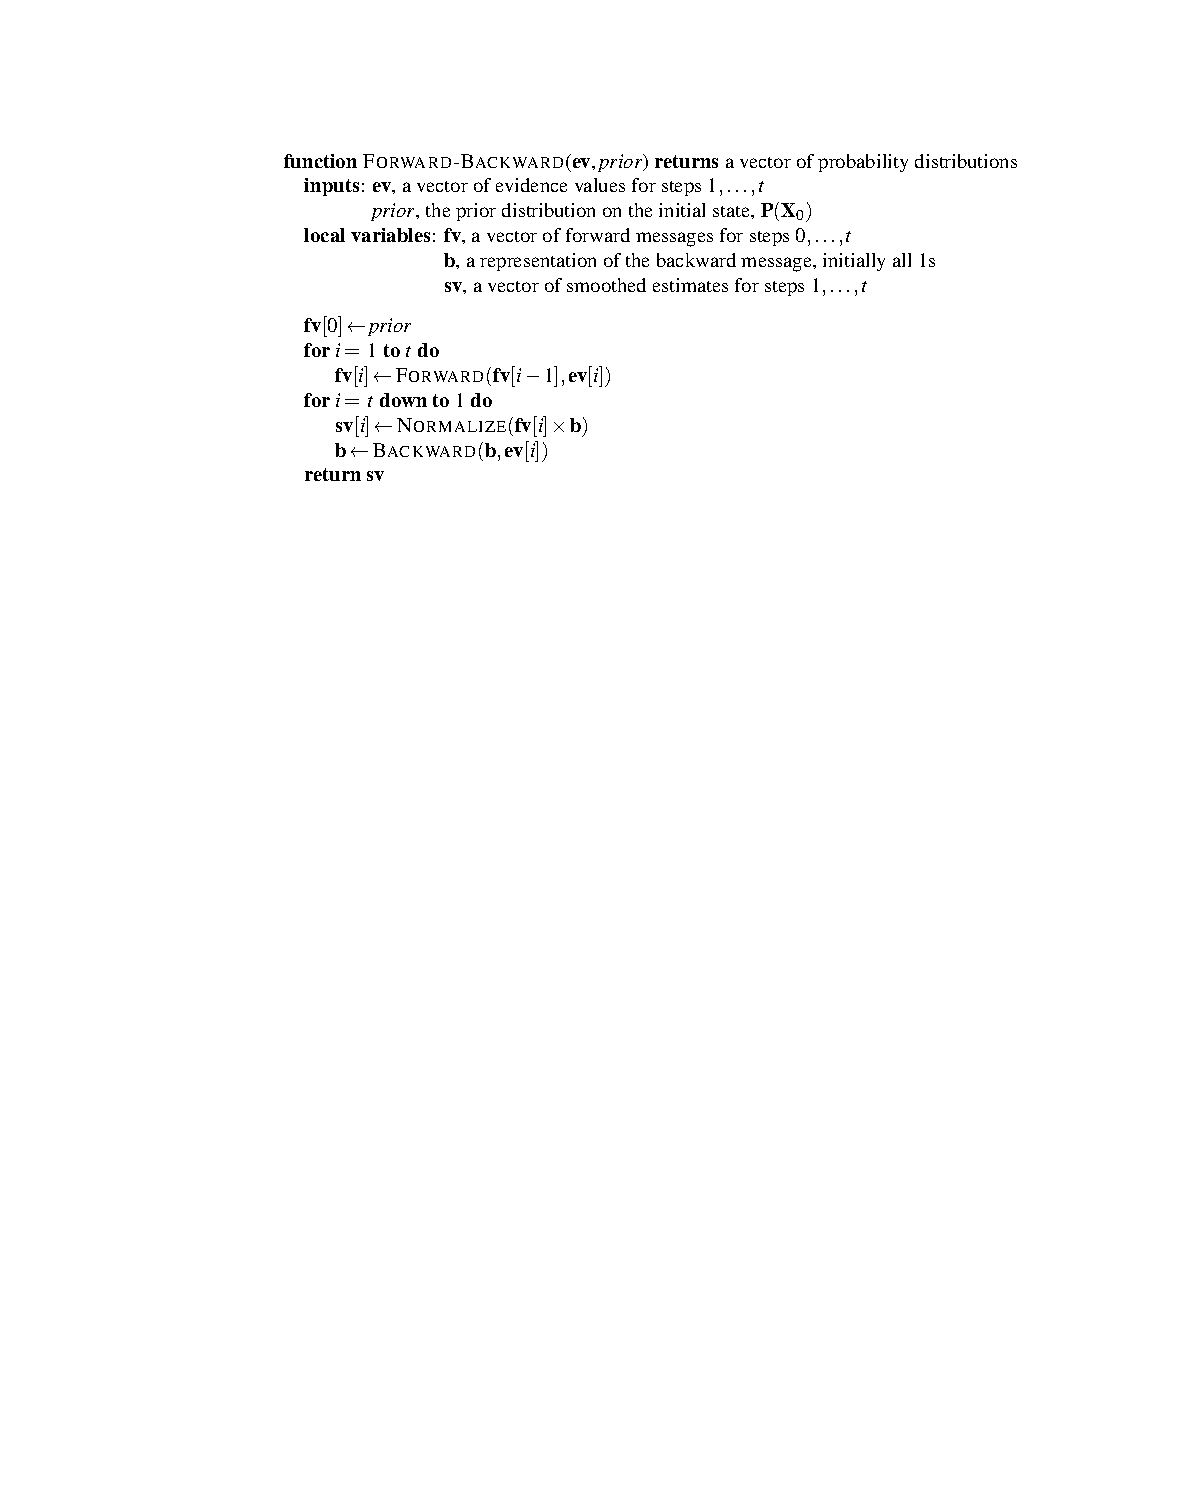
\includegraphics[alt={aima fig 14_04 forward backward algorithm},height=2.0in]{aima-fig-14_04-forward-backward-algorithm.pdf}


\(\text{FORWARD}(\bm{f}_{1:t}, \bm{e}_{t+1}) = P(\bm{X}_{t+1} \mid \bm{e}_{1:t+1}) =\)

\begin{itemize}
\item \(P(\bm{X}_{t+1} \mid \bm{e}_{1:t+1}) = \alpha P(\bm{e}_{t+1} \mid \bm{X}_{t+1}) \sum_{\bm{X}_t} P(\bm{X}_{t+1} \mid \bm{x}_t) P(\bm{x}_t \mid \bm{e}_{1:t})\) (14.5) and

\item the process begins with \(\bm{f}_{1:0} = P(\bm{X}_0)\).
\end{itemize}

\(\text{BACKWARD}(\bm{b}_{k+2:t}, \bm{e}_{k+1}) = P(\bm{e}_{k+1:t} \mid \bm{X}_k) =\)

\begin{itemize}
\item \(\sum_{\bm{x}_{k+1}} P(\bm{e}_{k+1} \mid \bm{x}_{k+1}) P(\bm{e}_{k+2:t} \mid \bm{x}_{k+1}) P(\bm{x}_{k+1} \mid \bm{X}_k)\) (14.9) and

\item initialize backward phase with \(\bm{b}_{t+1:t} = P(\bm{e}_{t+1:t} \mid \bm{X}_t) = \bm{1}\), where \(\bm{1} =\) vector of 1s.
\end{itemize}
\section{Inference in Temporal Models}
\label{sec:org1b10227}

Given the general structure of a probabilistic temporal model, we can perform basic inference tasks:

\begin{itemize}
\item \textbf{Filtering}, a.k.a., \textbf{state estimation} is the task of computing the \textbf{belief state} \(P(\bm{X}_t \mid \bm{e}_{1:t})\) -- the posterior distribution over the most recent state given all the evidence to date.

\item \textbf{Prediction} is the task of computing the posterior distribution over the future state, given all evidence to date: \(P(\bm{X}_{t+k} \mid \bm{e}_{1:t})\) for some \(k > 0\).

\item \textbf{Smoothing} is the task of computing the posterior distribution over a past state, given all evidence up to the present: \(P(\bm{X}_k \mid \bm{e}_{1:t})\) for some \(k\) such that \(0 \le k < t\).
\end{itemize}

\fbox\{
\begin{minipage}{\textwidth}
\begin{itemize}
\item {\bf Most likely explanation}: Given a sequence of observations, we might wish to find the sequence of states that is most likely to have generated those observations: $\argmax_{x_{1:t}} P(\bm{x}_{1:t} \mid \bm{e}_{1:t})$.
\end{itemize}
\end{minipage}
\}
\section{Finding the Most Likely Sequence}
\label{sec:org3c6c41c}

\textbf{Most likely explanation}: Given a sequence of observations, we might wish to find the sequence of states that is most likely to have generated those observations: \(\argmax_{x_{1:t}} P(\bm{x}_{1:t} \mid \bm{e}_{1:t})\).

\begin{itemize}
\item Umbrella example: if umbrella appears on each of the first three days and is absent on the fourth, then the most likely explanation is that it rained on the first three days and did not rain on the fourth.  On the other hand, perhaps the director forgot an umbrella on a rainy day, or took an umbrella on a sunny day out of caution.
\item MLE algorithms are useful for speech recognition -- where the aim is to find the most likely sequence of words, given a series of sounds, reconstruction of bit strings transmitted over a noisy channel, and many others.
\end{itemize}

We can represent the possible states in a system with a \textbf{state trellis}:


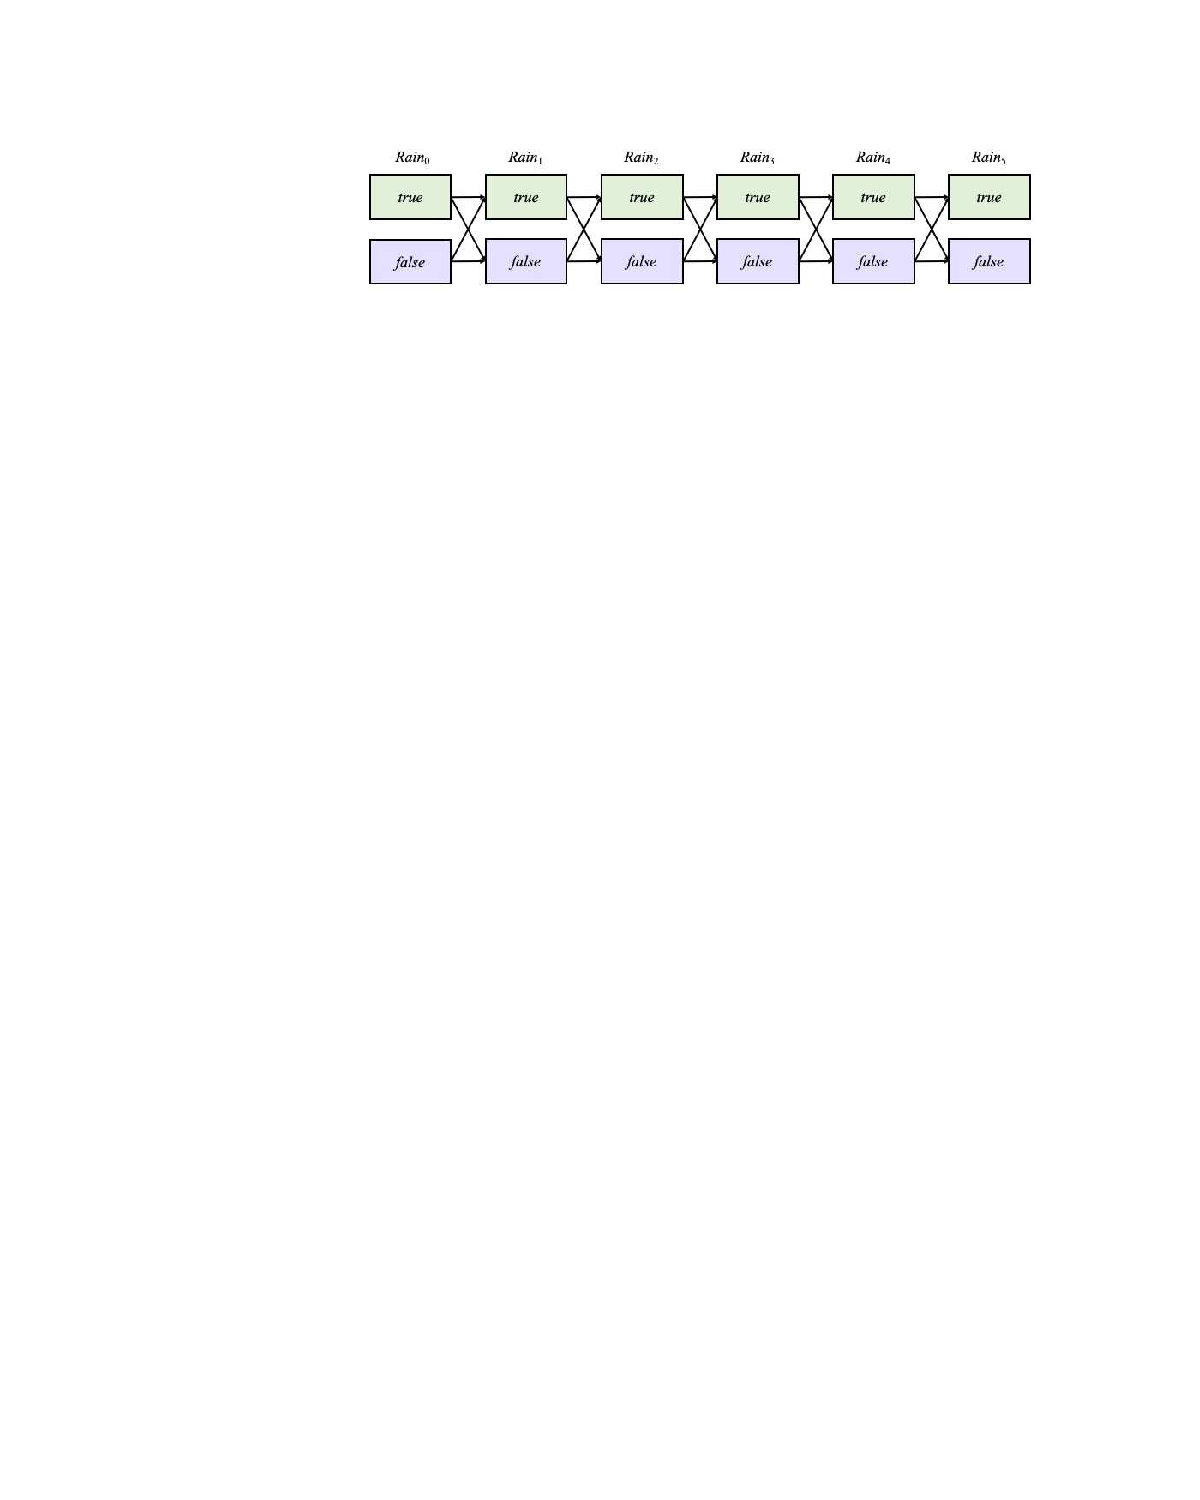
\includegraphics[alt={aima fig 14_05_a rain state trellis},width=0.75\linewidth]{aima-fig-14_05_a-rain-state-trellis.pdf}


Most likely sequence estimation is finding the most likely path through this graph, where the likelihood of any path is the product of the transition probabilities along the path and the probabilities of the given observations at each state.
\section{Most Likely Paths Through A State Trellis}
\label{sec:org3740e0c}


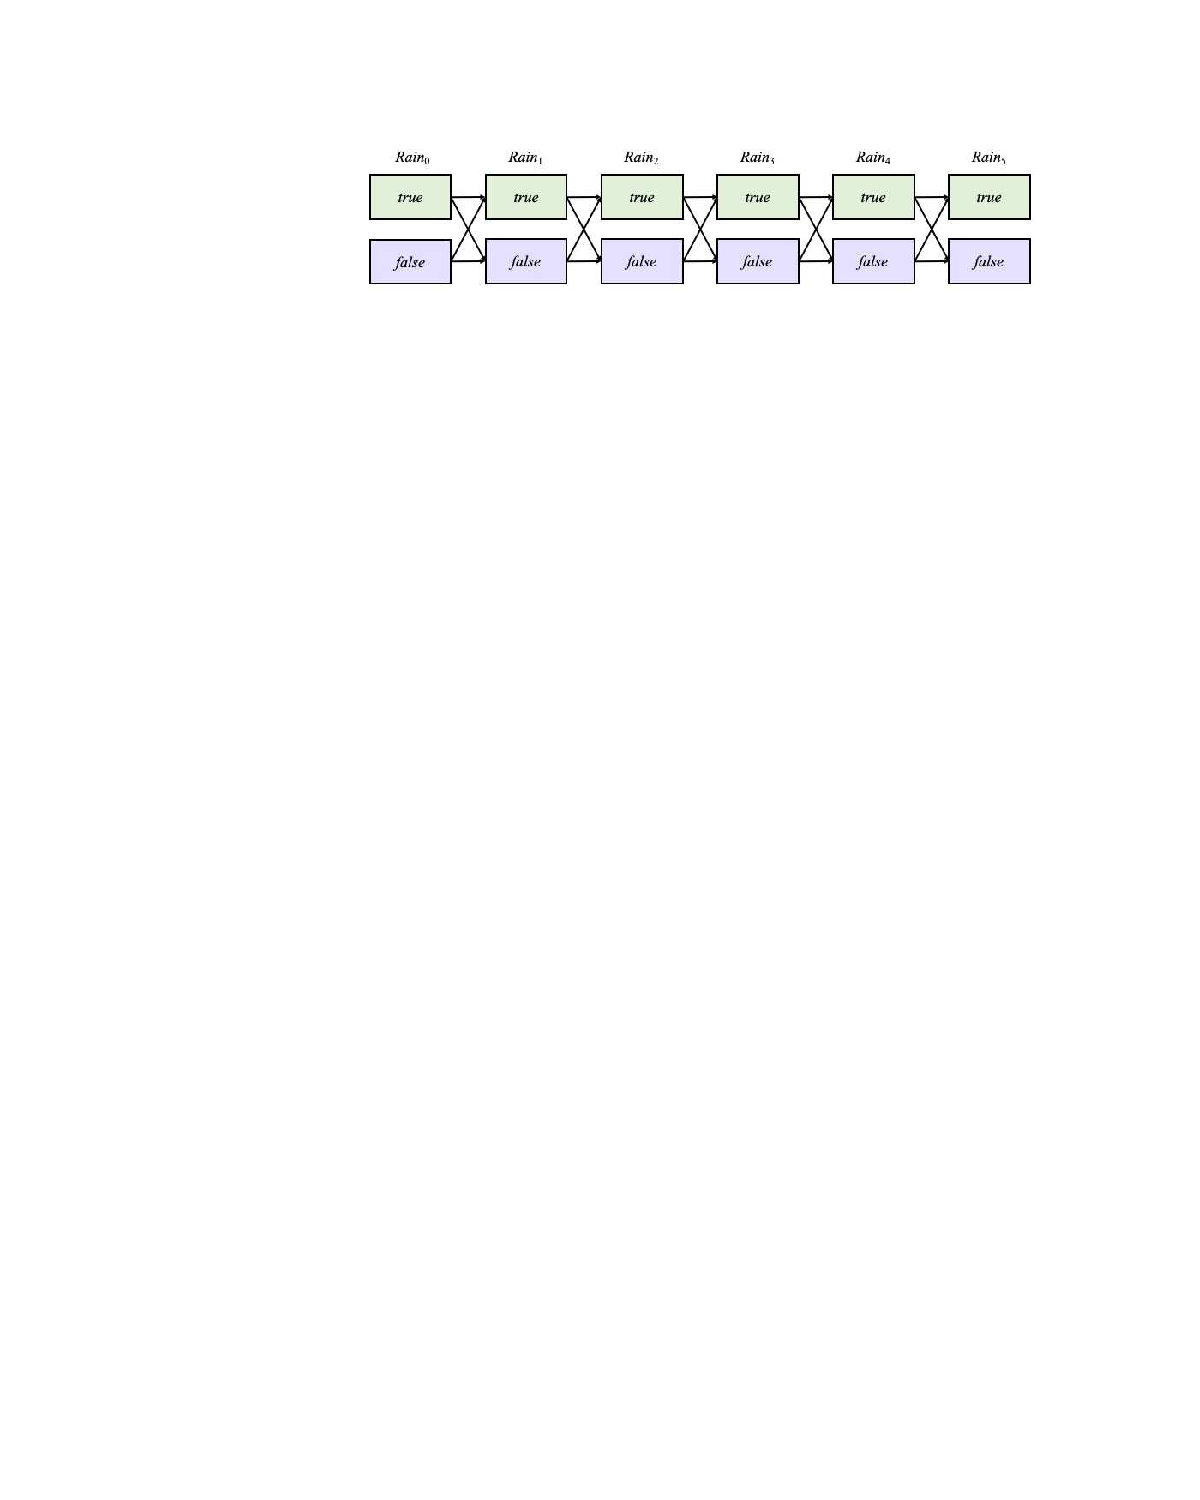
\includegraphics[alt={aima fig 14_05_a rain state trellis},width=0.75\linewidth]{aima-fig-14_05_a-rain-state-trellis.pdf}


Say we want to estimate the most likely path that reaches \(Rain_5 = true\).

\begin{itemize}
\item By the Markov property, the most likely path to \(Rain_5 = true\) consists of a path to a state at \(t=4\) followed by a transition to \(Rain_5 = true\).

\item The state at \(t = 4\) that becomes part of the path to \(Rain_5 = true\) is whichever state maximizes the likelihood of that path.
\end{itemize}

So there is a recursive relationship between most likely paths to each state \(\bm{x}_{t+1}\) and most likely paths to each state \(\bm{x}_{t}\).  We can use this property to construct a recursive algorithm for for computing the most likely path given the evidence.
\section{Viterbi Algorithm}
\label{sec:orgfe94216}

We will use a recursively computed message \(\bm{m}_{1:t}\), like the forward message \(\bm{f}_{1:t}\) in the filtering algorithm:

\begin{equation*}
\bm{m}_{1:t} = \max_{\bm{x}_{1:t}} P(\bm{x}_{1:t-1}, \bm{X}_t, \bm{e}_{1:t})
\end{equation*}

By applying a similar derivation to the one we used for the filtering equation (14.5), we get:

\begin{equation*}
\bm{m}_{1:t+1} = P(e_{t+1} \mid \bm{X}_{t+1}) \max_{\bm{x}_{t}} P(\bm{X}_{t+1} \mid \bm{x}_t) \max_{\bm{x}_{1:t-1}} P(\bm{x}_{1:t-1}, \bm{x}_{t}, \bm{e}_{1:t}) \tag{14.11}
\end{equation*}

\begin{itemize}
\item The final term \(P(\bm{x}_{1:t-1}, \bm{x}_{t}, \bm{e}_{1:t})\) is exactly the entry for the particular state \(\bm{x}_t\) in the message vector \(\bm{m}_{1:t}\).

\item Equation 14.11 is essentially identical to the filtering equation (14.5) except that the summation over \(\bm{x}_t\) in Equation (14.5) is replaced by the maximization over \(\bm{x}_t\) in Equation (14.11).

\item there is no normalization constant \(\alpha\) in Equation (14.11).
\end{itemize}

Thus, the algorithm for computing the most likely sequence is similar to filtering: it starts at time 0 with the prior \(\bm{m}_{1:0} = P(\bm{X}_0)\) and then runs forward along the sequence, computing the \(\bm{m}\) message at each time step using Equation (14.11).
\section{Operation of Viterbi Algorithm in Umbrella World}
\label{sec:orgd5b9c99}

Operation of the Viterbi algorithm for the umbrella observation sequence \([true,true,false,true,true]\), where the evidence starts at time 1.

\centering
\includegraphics{[}
    height=.4\textheight,
    alt=\{\}]
    \{aima-fig-14\textsubscript{05}\textsubscript{b}-viterbi-rain-state-probabilities.pdf\}

\begin{itemize}
\item For each \(t\), we show the values of the message \(\bm{m}_{1:t}\) , which gives the probability of the best sequence reaching each state at time t.

\item For each state, the bold arrow leading into it indicates its best predecessor as measured by the product of the preceding sequence probability and the transition probability.

\item Following the bold arrows back from the most likely state in \(\bm{m}_{1:5}\) gives the most likely sequence, shown by the bold outlines and darker shading.
\end{itemize}
\section{Practical computational considerations}
\label{sec:org592a732}

For longer sequences, likely to get floating point underflow.  Two solutions:

\begin{itemize}
\item Normalilze \(\bm{m}\) at each step.  Doesn't affect correctness because \(max(cx,cy) = c \cdot max(x,y)\).
\item Use log probabilities with addition in place of multiplication.  Correctness is
\end{itemize}
unaffected because the log function is monotonic, so \(max(\log x, \log y) = \log max(x,y)\)


Fun homework: \href{../../python/projects/markov-chains-recognition/markov-chains-recognition.html}{Markov Chains Recognition}
\end{document}
